\documentclass[1pt,letterpaper]{report}
\usepackage[utf8]{inputenc}
\usepackage[english]{babel}
\usepackage{amsmath}
\usepackage{amsfonts}
\usepackage{amssymb}
\usepackage[pdftex]{graphicx}
\usepackage{caption}
\usepackage{natbib}
\usepackage{enumerate}
\usepackage[pdftex,colorlinks,linkcolor=black,citecolor=black,filecolor=blue,urlcolor=blue]{hyperref}
\setcounter{section}{-1}
\usepackage{pdfpages}
\usepackage{natbib}
%
\usepackage{boxedminipage}
\usepackage{rotating}
\usepackage{tikz}
%\usepackage[left=0.1cm,right=0.1cm,top=.1cm,bottom=.1cm,papersize={230mm,196 mm}]{geometry}
\usepackage[left=0.1cm,right=0.1cm,top=.1cm,bottom=.1cm,papersize={213mm,261.5 mm}]{geometry}
\author{J. S. Castellanos-Dur\'an}
\setboolean{@twoside}{false}

\begin{document}
\sffamily
\graphicspath{{../Castellanos-Duran_et_al_2016/Figures/}}

\begin{picture}(600,240)
\put(-15,-74){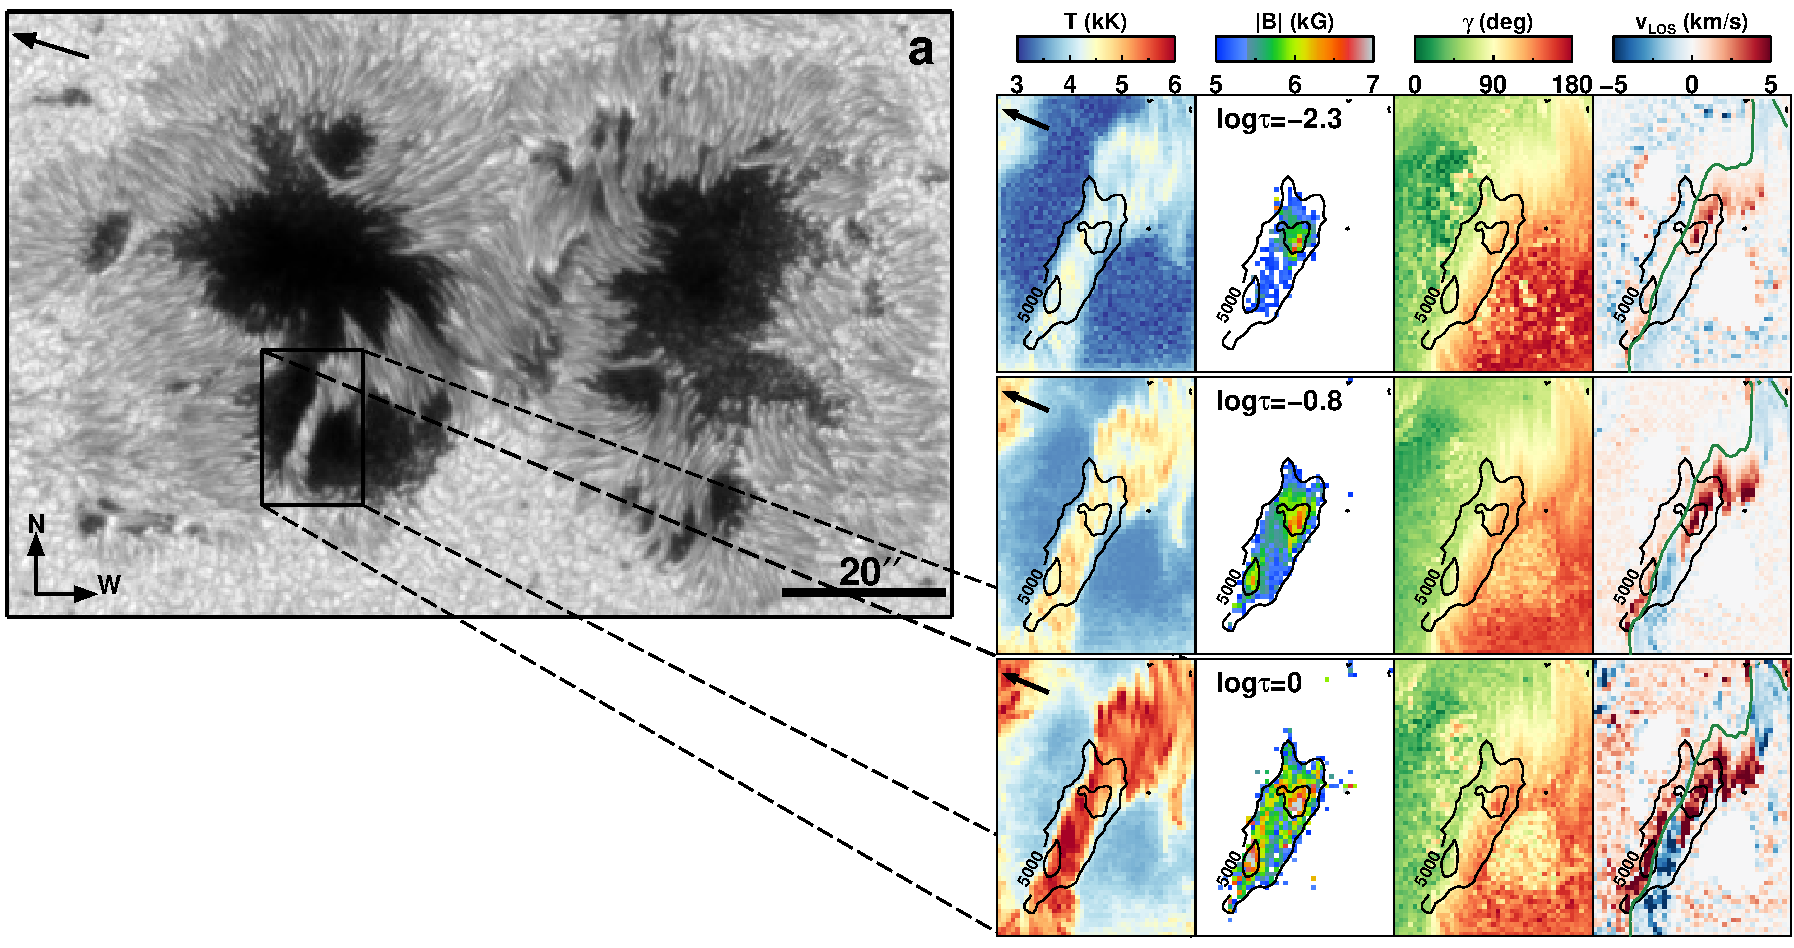
\includegraphics[width=1\textwidth]{Strong_fields_image_wedpage}}
\put(-15,-290){%
\begin{boxedminipage}{.998\textwidth}
\begin{huge}
\textbf{Abstract:} Traditionally, the strongest magnetic fields on the Sun have been measured in sunspot umbrae. More recently, however,  much stronger fields have been measured at the ends of penumbral filaments carrying the Evershed and Counter-Evershed flows. Superstrong fields have also been reported within a light bridge separating two umbrae of opposite polarities. We aim to accurately determine the strengths of the strongest fields in a light bridge using an advanced inversion technique and to investigate their detailed structure. We analyze observations from the spectropolarimeter on board the Hinode spacecraft of the active region AR 11967. The thermodynamic and magnetic configurations are obtained by inverting the Stokes profiles using an inversion scheme that allows multiple height nodes. \textbf{Both the traditional 1D inversion technique and the so-called 2D coupled inversions, which take into account the point spread function of the Hinode telescope, are used.} We find a compact structure with an area of 32.7 arcsec$^2$ within a bipolar light bridge with field strengths exceeding 5\,kG, confirming the strong fields in this light bridge reported in the literature. \textbf{Two regions associated with downflows of $\sim$5\,km\,s$^{-1}$ harbor field strengths larger than 6.5\,kG, covering a total area of 2.97 arcsec$^2$. The maximum field strength found is 8.2\,kG, which is the largest ever observed field in a bipolar light bridge up to now. }
\end{huge}
\end{boxedminipage}}
\end{picture}







\end{document}